\documentclass[a4paper, 12pt]{article}
\usepackage{graphicx, subfig}
\usepackage{amsmath,amsfonts,amssymb,amsthm, mathtools, commath}
\usepackage{lscape,tabularx,booktabs}
\usepackage{color,soul}
\usepackage{fullpage} 
\usepackage{natbib}
\usepackage{pdfpages}
\usepackage[utf8]{inputenc}
\usepackage[english]{babel}
\usepackage[top=1.25in, left=1.25in, right=1.25in, bottom=1.25in]{geometry}

\newcommand{\ubar}[1]{\text{\b{$#1$}}} 

\usepackage{pgfplots}
\usepgfplotslibrary{polar}
\usepgflibrary{shapes.geometric}
\usetikzlibrary{calc}
\pgfplotsset{compat=1.16}

\setlength{\parindent}{2em}
\setlength{\parskip}{0.5em}

\begin{document}

\begin{center}
    \Large \textbf{UT IO VM Computational Experiments}  \\
    Nathan Hattersley, Justin Latona, and Hayden Parsley 
\end{center}


\subsection{September 14th, 2023}

We've taken the data from Dan's Rust homework assignment and have replicated it such that we're left with a data set of size 1000, 10000, ..., 1000000. For each data set of size $N$ we execute code that evaluates a single objective function call in Julia, Matlab, and Python. We have written code to evaluate the likelihood in three different ways; 
\begin{enumerate}
    \item Serial Implementation - a for loop through each observation that assigns the respective CCP value given the observed action of the agent 
    \item Explicit Parallel Implementation - we replace the for loop with a parallelized version using different number of processors 
    \item Implicit Parallel Implementation - a vectorized implementation that takes advantage of each language's implicit parallelization sub routines 
\end{enumerate}

We present the relative gains of explicit parallelization (explicit parallel runtime/serial runtime) for each programming language first. This means a value less than one, implies that the parallelized version of the for-loop is faster than the serial for-loop. 

\begin{figure}[!ht]
    \centering
    \caption{Julia - Relative Explicit Parallel Performance}
    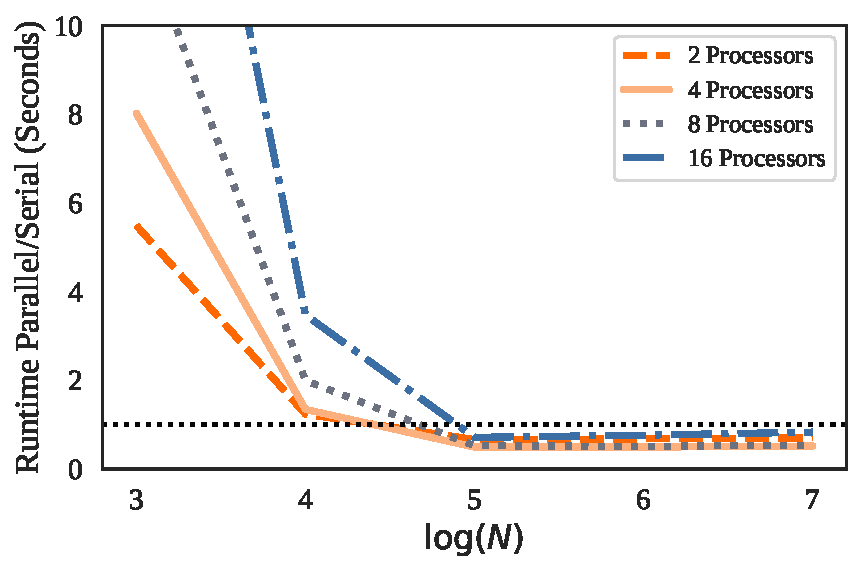
\includegraphics[scale = 0.75]{../figs/juliaNormParFor.pdf}
\end{figure}


\begin{figure}[!ht]
    \centering
    \caption{Matlab - Relative Explicit Parallel Performance}
    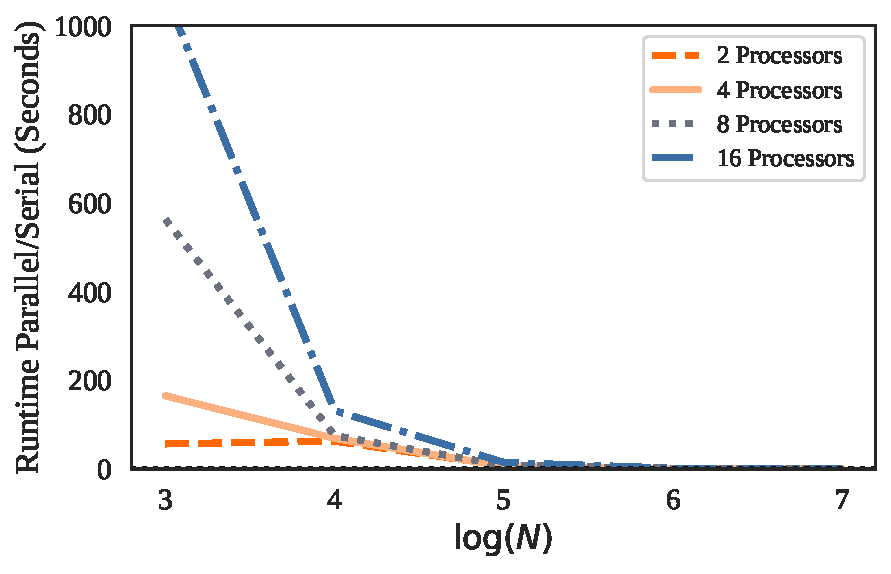
\includegraphics[scale = 0.75]{../figs/matlabNormParFor.pdf}
\end{figure}


\begin{figure}[!ht]
    \centering
    \caption{Python - Relative Explicit Parallel Performance}
    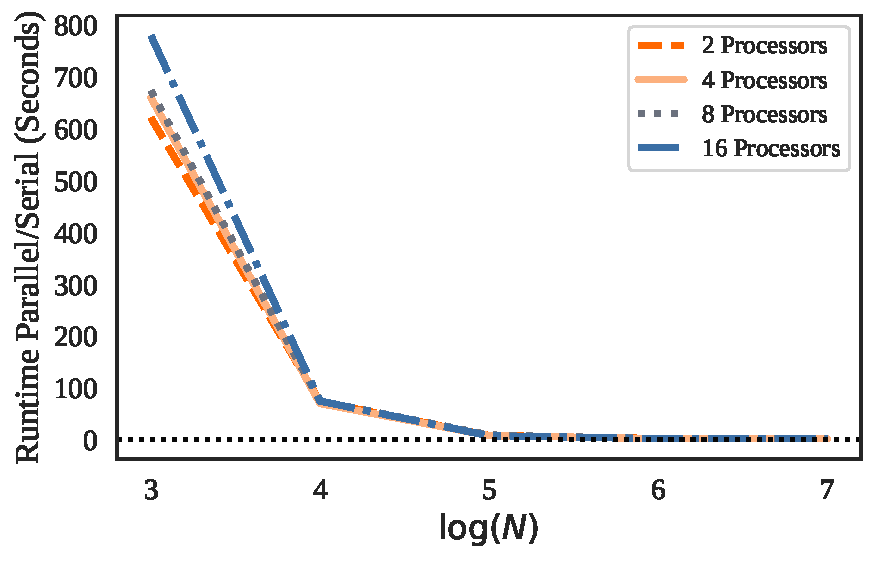
\includegraphics[scale = 0.75]{../figs/pythonNormParFor.pdf}
\end{figure}

\pagebreak 

A couple of notes; 

\begin{itemize}
    \item Julia is the fastest in terms of run time for both the serial and explicit parallelization, followed by Matlab and then Python. 
    \item Julia seems to be the only language of the three that can get a speed up with the explicit parallelization procedure. Matlab seems some gains, but only for the largest data sets. Python's explicit parallelization implementation always seems to do worse than the serial implementation. 
    \item Matlab appears to have the largest ``start-up'' costs when it comes to explicit parallelization. All languages have a higher fixed cost of starting the parallelization as the number of processors increase. 
\end{itemize}

We next present the implicit parallelization procedure both in levels and the relative performance compared to the explicit parallelization procedures across the three languages, 


\begin{figure}[!ht]
    \centering
    \caption{Implicit Parallel Performance}
    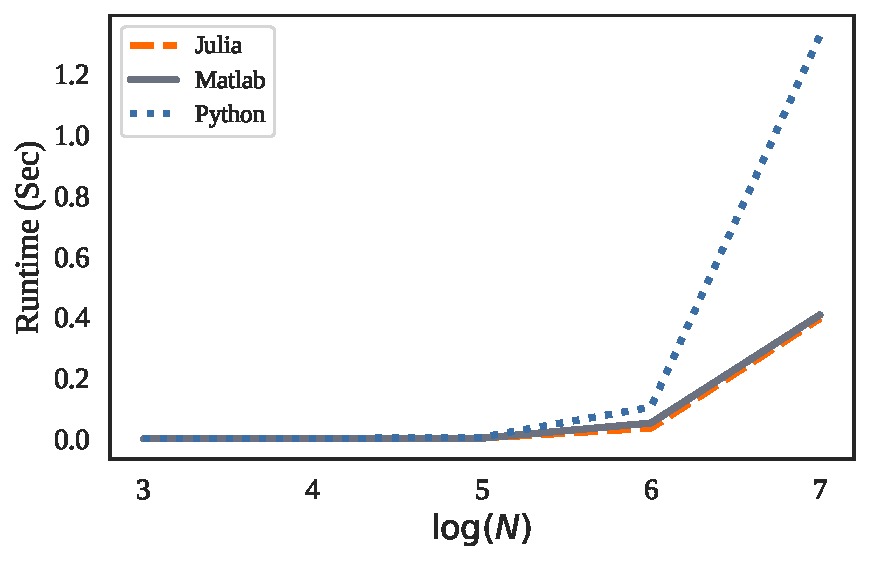
\includegraphics[scale = 0.75]{../figs/vectorizedRT.pdf}
\end{figure}


\begin{figure}[!ht]
    \centering
    \caption{Relative Implicit Parallel Performance}
    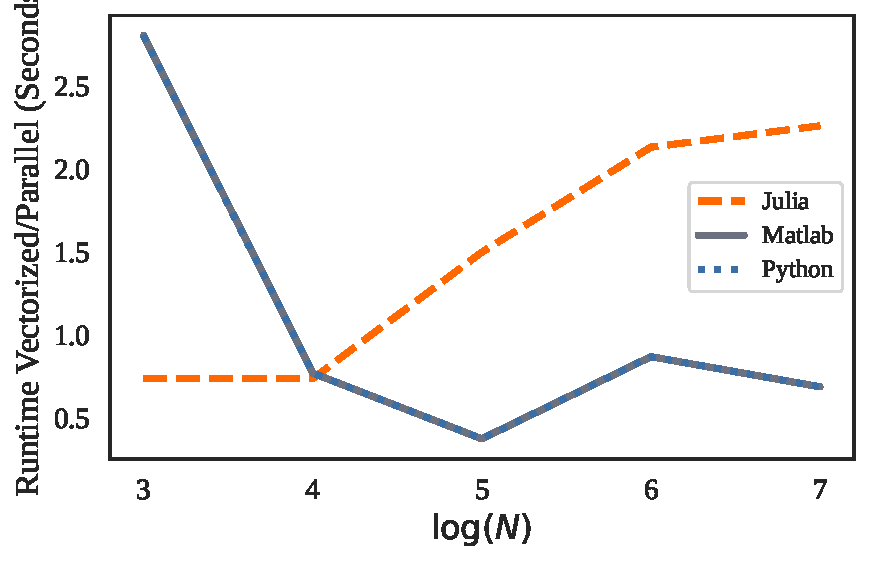
\includegraphics[scale = 0.75]{../figs/vectorizedNormRT.pdf}
\end{figure}

Runtimes are rather close -- speaks to them using similar fortran binaries to do these operations. Almost surely for Python and Matlab, the vectorized implementation is faster than the parallel implementation. In Julia, there seems to be some tradeoffs. 

\end{document}